\documentclass[tikz,border=8pt]{standalone}
\usetikzlibrary{angles,calc,quotes}

\begin{document}
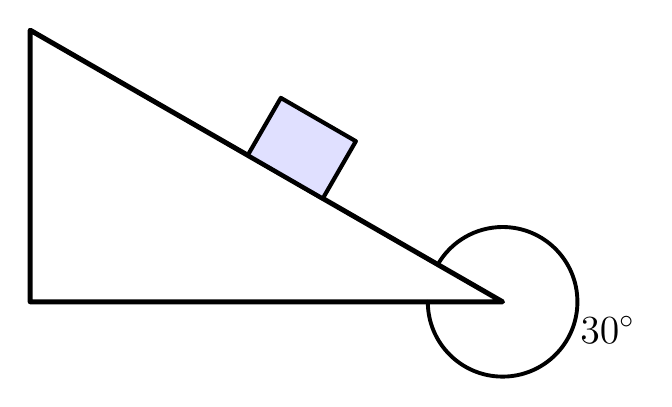
\begin{tikzpicture}[
  line cap=round,
  line join=round,
  every node/.style={font=\Large}
]
  \coordinate (A) at (0,0);
  \coordinate (B) at (6,0);
  \coordinate (C) at (0,3.45);

  \draw[line width=1.8pt] (A) -- (B) -- (C) -- cycle;
  \pic[
    draw,
    line width=1.4pt,
    angle radius=0.95cm,
    angle eccentricity=1.45,
    "$30^\circ$"
  ] {angle=A--B--C};

  \begin{scope}[shift={($(B)!0.46!(C)$)}, rotate=-30]
    \draw[line width=1.5pt, fill=blue!12] (-0.55,0) rectangle (0.55,0.84);
  \end{scope}
\end{tikzpicture}
\end{document}
